% 6.1.2 Applikationsmodeller
\subsection{Applikationsmodeller}

Selve designet af softwaren bygger på de følgende applikationsmodeller. Her laves der sekvens- og klassediagrammer over hver del af systemet samt klassebeskrivelser, hvor funktionen for de enkelte metoder beskrives.

% 6.1.2.1 DevKit8000
\subsubsection{DevKit8000}

Applikationsmodel for UC1: Kalibrer system.

\begin{figure}[H] \centering
    \fbox{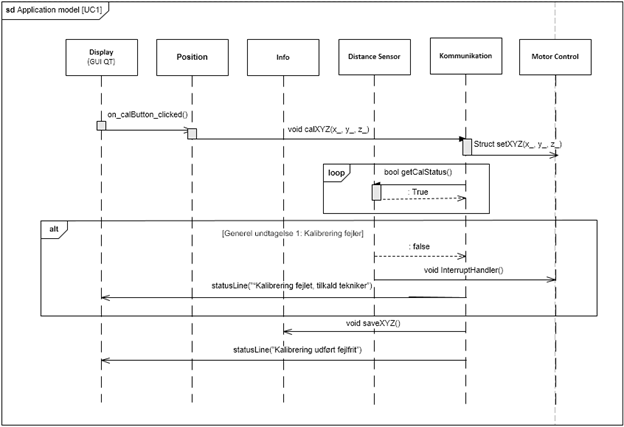
\includegraphics[width=0.95\textwidth]{0_Filer/Figuer/uc1App.png}}
    \caption{Applikationsmodel med udgangspunkt i UC1}
    \label{fig:uc1App}
\end{figure}

\begin{figure}[H] \centering
    \fbox{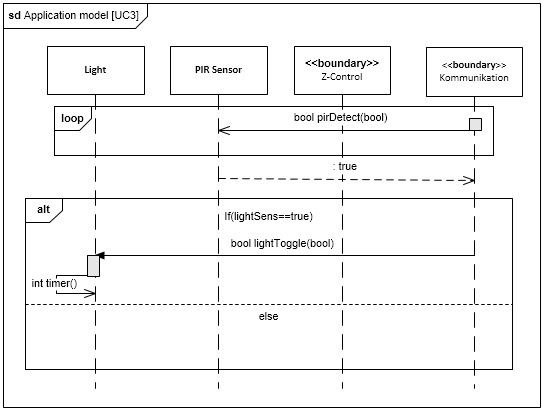
\includegraphics[width=0.95\textwidth]{0_Filer/Figuer/uc3App.png}}
    \caption{Applikationsmodel med udgangspunkt i UC3}
    \label{fig:uc3App}
\end{figure}


% 6.1.2.2 PSoC Master
\subsubsection{PSoC Master}

Applikationsmodeller for PSoC Master.

\begin{figure}[H] \centering
    \fbox{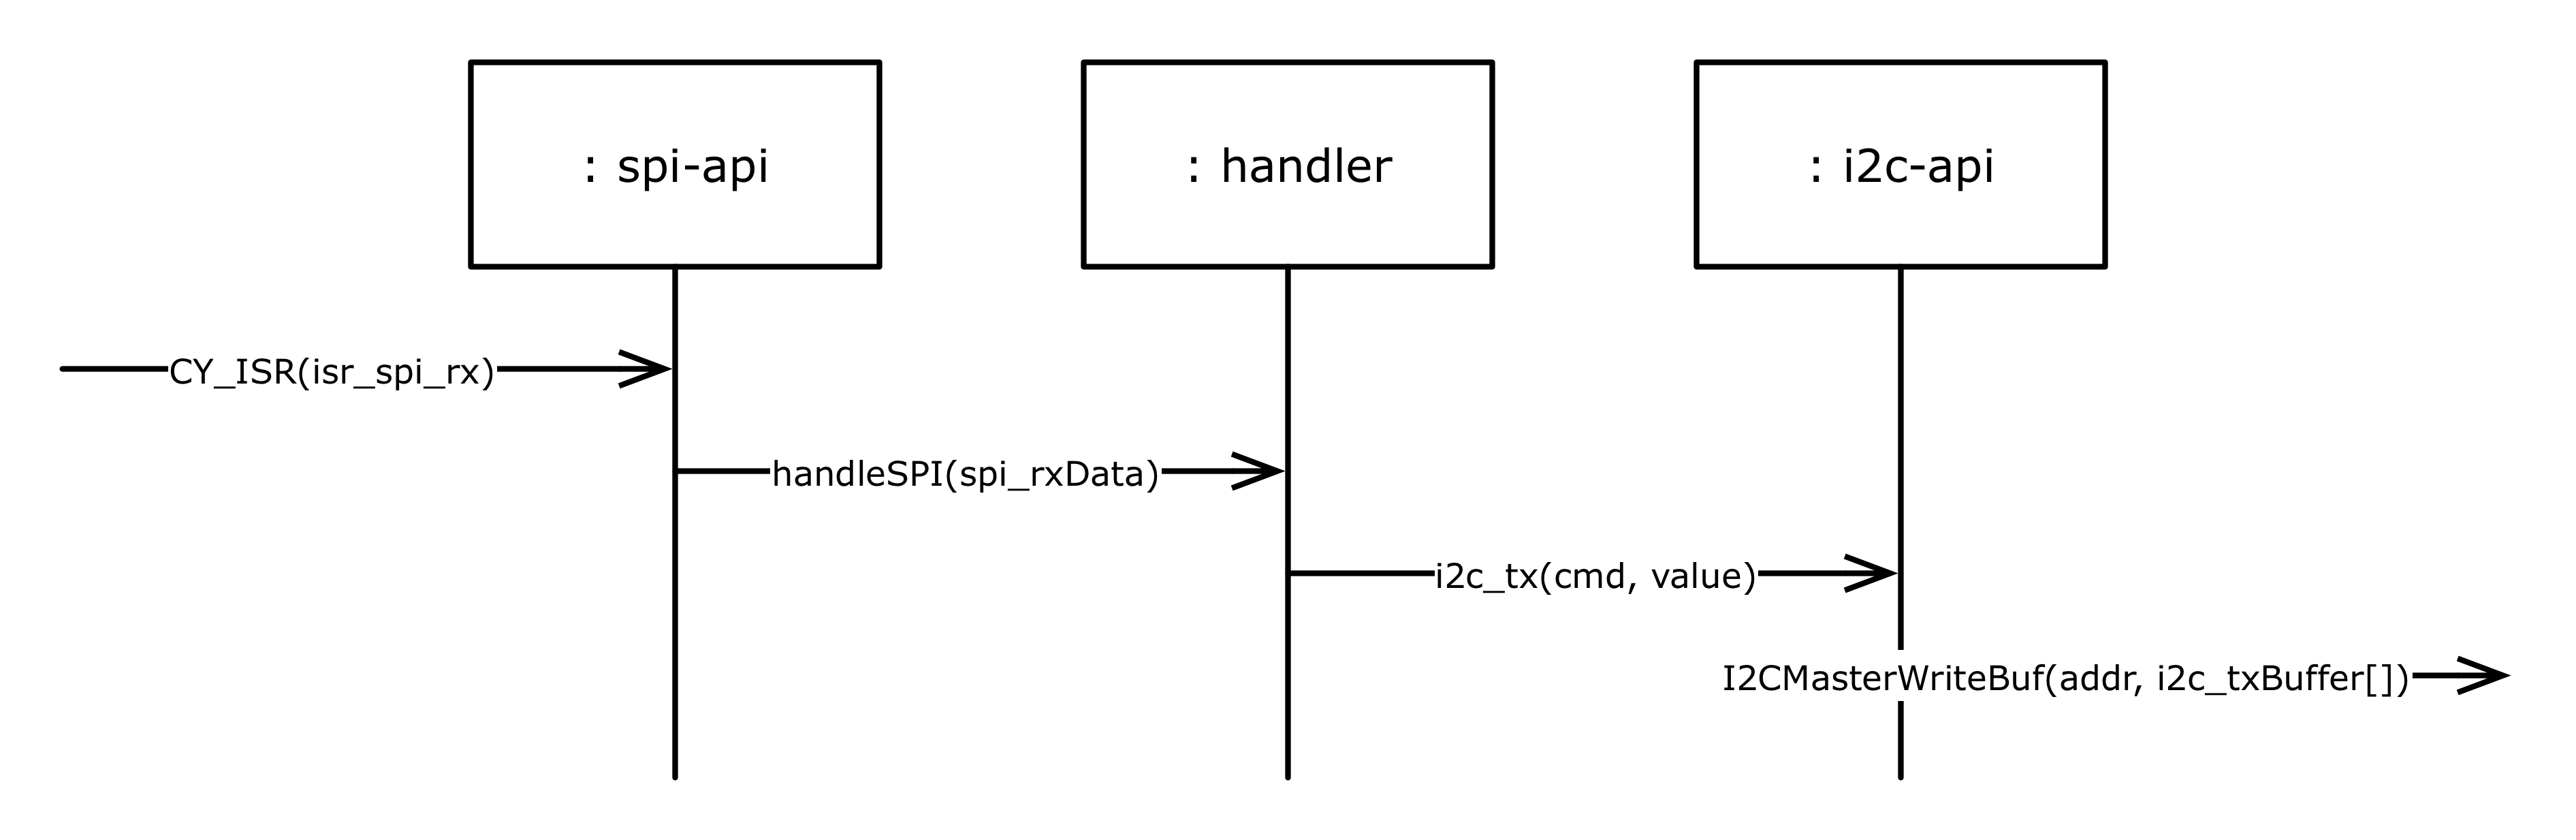
\includegraphics[width=0.95\textwidth]{0_Filer/Figuer/SPItoI2C.png}}
    \caption{Sekvensdiagram for "set" kommando via PSoC Master}
    \label{fig:sekvensdiagram_psoc_master_set}
\end{figure}

\begin{figure}[H] \centering
    \fbox{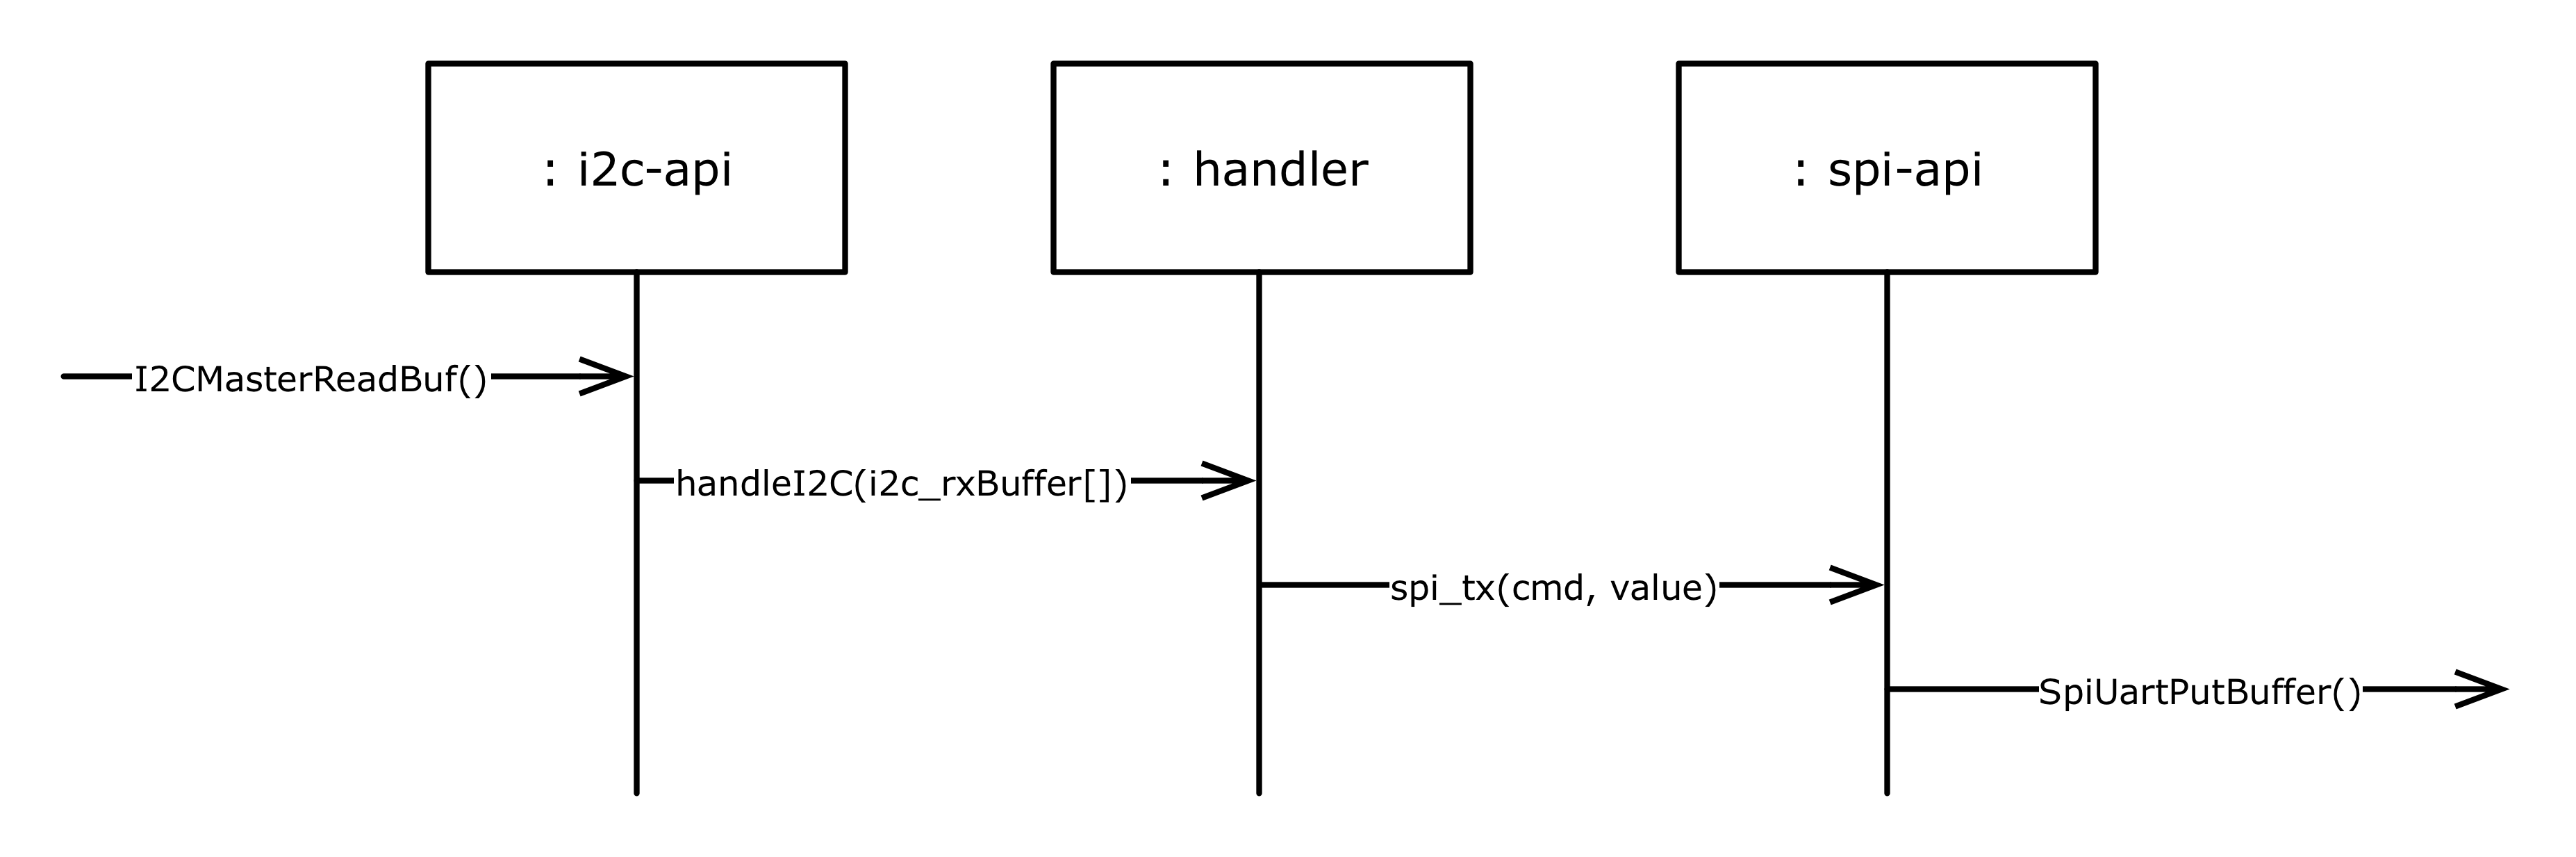
\includegraphics[width=0.95\textwidth]{0_Filer/Figuer/I2CtoSPI.png}}
    \caption{Sekvensdiagram for "get" kommando via PSoC Master}
    \label{fig:sekvensdiagram_psoc_master_get}
\end{figure}

% 6.1.2.3 Klassebeskrivelser
\subsubsection{Klassebeskrivelser PSoC Master}

Her følger klassebeskrivelser for de udledte klasser fra applikationsmodellerne.
% 6.1.2.3 Klassebeskrivelser PSoC Master

% spi-api
\begin{table}[H]
    \centering
    \begin{tabular}{|l|}
    \hline
    \multicolumn{1}{|c|}{<<boundary>>} \\
    \multicolumn{1}{|c|}{\textbf{SPI-API}} \\
    \hline
    - uint16 spi\_rxData \\
    - uint16 spi\_txData \\
    \hline
    + spi\_init() :void \\
    + spi\_tx(uint16) : void \\
    + CY\_ISR(isr\_spi\_rx) \\
    \hline
    \end{tabular}
    \caption{Klassen SPI-API på PSoC-Master}
    \label{tab:classSpiApiPSoCMaster}
\end{table}

{\centering\textbf{spi-api (PSoC Master)}\par}

\begin{labeling}{Attributter:}
\item[Ansvar:] At håndtere spi kommuniaktionen mellem DevKit og PSoC Master.
\item[Attributter:] uint16 spi\_rxData \\
uint16 spi\_txData
\end{labeling}

\begin{labeling}{Beskrivelse:}
\item[void spi\_init()]
\item[Parametre:] Ingen.
\item [Returværdi:] Ingen.
\item [Beskrivelse:] Initialsere SPI komponentet på PSoC Master.
\end{labeling}

\begin{labeling}{Beskrivelse:}
\item[void spi\_tx(uint16)]
\item[Parametre:] Modtager en unsigned int 16.
\item [Returværdi:] Ingen.
\item [Beskrivelse:] Metoden modtager en unsigned int på 16-bit, som den lægger klar til anvendelse via SPI kommuniaktionen til DevKit ved næste ledige bus tid.
\end{labeling}

\begin{labeling}{Beskrivelse:}
\item[CY\_ISR(isr\_spi\_rx)]
\item[Parametre:] Navnet på isr funktionen.
\item [Returværdi:] Ingen.
\item [Beskrivelse:] Metoden opretter en isr som klades automatisk, når der bliver sendt data til PSoC Master via spi kommuniaktionen.
\end{labeling}

% handler
\begin{table}[H]
    \centering
    \begin{tabular}{|l|}
    \hline
    \multicolumn{1}{|c|}{<<controler>>} \\
    \multicolumn{1}{|c|}{\textbf{handler}} \\
    \hline
    \\
    \hline
    + handleSPI(uint8, uint16) : void \\
    + handleI2C(uint8, uint16) : void \\
    \hline
    \end{tabular}
    \caption{Klassen handler på PSoC-Master}
    \label{tab:classHandlerPSoCMaster}
\end{table}

{\centering\textbf{handler (PSoC-Master)}\par}

\begin{labeling}{Attributter:}
\item[Ansvar:] At håndtere alt data flow på PSoC Master.
\item[Attributter:] ingen.
\end{labeling}

\begin{labeling}{Beskrivelse:}
\item[void handleSPI(uint8, uint16)]
\item[Parametre:] Modtager en unsigned int 8 og en unsigned int 16.
\item [Returværdi:] Ingen.
\item [Beskrivelse:] Metoden modtager en unsigned int på 8-bit, som indholder en kommandoen, der håndteres og en tilhørende unsigned int på 16-bit, som indholder en værdi.
\end{labeling}

\begin{labeling}{Beskrivelse:}
\item[void handleI2C()]
\item[Parametre:]Modtager en unsigned int 8 og en unsigned int 16.
\item [Returværdi:] Ingen.
\item [Beskrivelse:] Metoden modtager en unsigned int på 8-bit som indholder en kommandon som håndteres og en tilhørende unsigned int på 16-bit som indholder en værdi.
\end{labeling}

% I2C-API
\begin{table}[H]
    \centering
    \begin{tabular}{|l|}
    \hline
    \multicolumn{1}{|c|}{<<boundary>>} \\
    \multicolumn{1}{|c|}{\textbf{I2C-API}} \\
    \hline
    - uint8 i2c\_txBuffer[] \\
    - uint8 i2c\_txBuffer[] \\
    \hline
    + i2c\_init() : void \\
    + i2c\_tx() : void \\
    + i2c\_rx() : void \\
    \hline
    \end{tabular}
    \caption{Klassen I2C-API på PSoC Master}
    \label{tab:classI2cApiPSoCMaster}
\end{table}

{\centering\textbf{I2C-API (PSoC Master)}\par}

\begin{labeling}{Attributter:}
\item[Ansvar:] At håndtere I2C kommuniaktionen mellem PSoC-Master og PSoC-XY, PSoC-Z og PSoC-Sensor.
\item[Attributter:] uint8 i2c\_txBuffer[]\\
uint8 i2c\_txBuffer[]
\end{labeling}

\begin{labeling}{Beskrivelse:}
\item[void i2c\_init()]
\item[Parametre:] Ingen.
\item [Returværdi:] Ingen.
\item [Beskrivelse:] Initialsere I2C komponentet på PSoC Master.
\end{labeling}

\begin{labeling}{Beskrivelse:}
\item[void i2c\_tx(uint16)]
\item[Parametre:] Modtager en unsigned int 16.
\item [Returværdi:] Ingen.
\item [Beskrivelse:] Metoden modtager en unsigned int på 16-bit, som den lægger klar til anvendelse via I2C kommuniaktionen.
\end{labeling}

\begin{labeling}{Beskrivelse:}
\item[void i2c\_rx(uint16)]
\item[Parametre:] Modtager en unsigned int 16.
\item [Returværdi:] Ingen.
\item [Beskrivelse:] Metoden modtager en unsigned int på 16-bit, som den lægger klar til anvendelse via I2C kommuniaktionen.
\end{labeling}



\subsubsection{PSoC-Sensor arkitektur og implementering}

På TopDesign niveau består PSoC-Sensor af 7 blokke:
\begin{itemize}
	\item Afstandssensor
	\item PIR sensor
    \item Lumen sensor
	\item LED PWM
	\item Intern kommunikation
	\item Main lop metronom
	\item Debug
\end{itemize}

For at aflæse afstandssensoren skal vi kunne måle hvor længe en pin bliver holdt høj, med en præcision på et par mikrosekunder (1 cm svare til 58 us). Derfor har vi sat en timer op med en 1 MHz clock, der starter med at tælle på rising edge af det signal der skal måles, og derefter stopper, gemmer tællerværdien og starter en interrupt på falling edge. 

Denne blok har desuden tre ekstra pins: DistTrigger, DistReset, og DistInterruptPin. DistTrigger bruges til at starte målingen - sensoren skal have en 10 us puls som input før den starter. DistReset bruges til at resette timeren mellem målingerne, da den ellers blot fortsætter med at tælle derfra hvor den kom til. Til sidst bruges DistInterruptPin til at sende et signal direkte til PSoC-Z når afstandssensoren måler at vi er kommet for tæt på en underliggende forhindring.

PIR sensor blokken er noget simplere: Sensoren holder et output højt når den detekterer bevægelse og lavt ellers, så der behøves blot en pin til at aflæse det signal.

Lyssensoren kommunikere over I2C, så her behøves kun et I2C Master modul.

De tre LEDs styres med PWM, og hver farve (rød, grøn, blå) har sit eget PWM modul. De deler dog alle tre clock med afstandssensor-timeren. Dette er valgt fordi PSoC4 maksimalt understøtter fire brugerdefinerede clocks, så når forskellige komponenter kan sættes til at virke med samme clock-frekvens, er der ingen grund til at bruge flere resourcer end nødvendigt.

Den interne kommunikation mellem PSoCs foregår med I2C protokollen, men i det her tilfælde er Sensor-PSoC en slave.

Den næstsidste blok er Metronomen. Den indeholder en timer der er sat til at lave et interrupt hvert halve sekund. De interrupts bliver så brugt i hovedprogrammet til at aktiverer sensoraflæsninger og andre periodiske events. Denne timer har sin egen clock (200 Hz), da det gjorde designet nemmere og lod os holde timeren på 8 bits, hvilket spare andre resourcer i PSoC'en.

Den sidste blok er Debug. Den indeholder et UART modul, men da de to I2C moduler optager alle de dedikerede hardware kommunikationsblokke, så der bliver her brugt et software modul der kun understøter transmit.

{\centering\textbf{PSoC-Sensor implementering}\par}

I softwaren findes der disse filer:
\begin{itemize}
	\item SensorData
	\item CircularMean
	\item i2c
	\item queue
	\item handler
	\item LumenSensor
	\item lux
	\item main
\end{itemize}

\textbf{SensorData} har en struct der indeholder alle de globale sensor data og instillinger systemet bruger, samt en init funktion der sætter værdierne til noget fornuftigt under opstart.

\textbf{CircularMean} er datastruktur der kun kan modtage integer data og returnerer en gennemsnitlig værdi for de sidste X indsatte værdier. Så den er lidt dårligt navngivet og burde have heddet CircularAverage. Den er implementeret med et array der bliver indekseret fortløbende indtil enden bliver nået, hvorefter skrive-pointeren bliver nulstillet og de ældste værdier begynder at blive overskrevet.

\textbf{i2c} og \textbf{queue} er de moduler der håndterer I2C kommunikationen. Disse moduler er nærmere beskrævet i TODO: INSERT-REFERENCE

Modulet \textbf{handler} håndterer PSoC-Sensors opførsel når den modtager I2C kommandoer fra PSoC-Master. Den er implementeret med en stor switch, med en case for hver kommando PSoC-Sensor kan modtage og håndterer. Desuden har modulet en debug funktion, hvor man ved at aktiverer en \#define kan få alle modtagne kommandoer udskrevet på debug uart forbindelsen.

\textbf{LumenSensor} er det software modul der håndterer I2C kommunikationen med lyssensoren. Dette har fået sit eget modul da en enkelt aflæsning af sensoren består af at skrive en byte til sensoren, læse to bytes fra sensoren, og derefter skrive en og læse to bytes igen. Denne kommunikation bruger \texttt{NO\_STOP} og \texttt{REPEAT\_START} flagende, hvilket gør at alle fire dataoverførsler teknisk set foregår i en I2C kommunikation. Dette betyder ikke noget her da der kun er en master og en slave på linjen, men i et større system vil det forhindre en anden master i at tage linjen i det splitsekund hvor den bliver frigivet. Derudover spare man også omkring 3 bits på linjen på de udeblivende stop.

\textbf{lux} modulet er ikke noget vi har skrevet selv. De målinger lyssensoren giver bør køres gennem en formel der som resultat giver et rimeligt tal for den mængde synligt lys sensoren kan se, i måleenheden lux. Denne formel er beskrevet i sensorens datablad, og databladet indeholder desuden en færtig C-funktion der kan udføre beregningen hurtigt og effektivt på en mikroprocessor. Det er denne C-funktion vi har kopieret over i lux modulet.

Sidst men ikke mindst er der \textbf{main}. Den indeholder den overordnede kontrolstruktur i PSoC-Sensor, der bestemmer hvornår alt andet skal køres. Som beskrevet ovenfor i TopDesign, så er hjertet Metronom timeren der giver et taktslag hver halve sekund. For hvert taktslag bliver en række tællere talt op og tjekket for overløb. Hver tæller der løber over bliver nulstillet og hæver et flag. De flag bliver så tjekket i hovedløkken og den tilhørende kode bliver udført.

Alt i alt giver denne opbygning at der kan defineres periodiske events med individuelle perioder (med en opløsning på 0.5 sekunder). Det giver den fordel at vi kan have en hoved-løkke der kører hele tiden, uden at blive standset af delay kommandoer, hvilket giver muligheden for et mere responsiv og jævnt kørende program. Men samtidig undgår vi at overbelaste sensorene ved at aktiverer dem alt for ofte.

Selve kontrolstrukturen er implementeret med et dobbelt array:

\begin{lstlisting}[frame=single, basicstyle=\footnotesize\ttfamily, language=C, numbers=left, numberstyle=\tiny\color{black}, caption={Kodeudsnit: controlFlags},captionpos=b]
char controlFlags[5][3] = {
    {1,-1, 0},
    {1,-1, 0},
    {1,-1, 0},
    {1,-1, 0},
    {1,-1, 0}
};
\end{lstlisting}

Men for at gøre koden mere læsevenlig, så bliver arrayet kun indekseret med enum navne. Det har også den fordel at hvis der skal oprettes et nyt periodisk event, så behøver man kun kopierer en ekstra linje ind i arrayet, og tilføje et navn til en enum liste.

\begin{lstlisting}[frame=single, basicstyle=\footnotesize\ttfamily, language=C, numbers=left, numberstyle=\tiny\color{black}, caption={Kodeudsnit: enums og indeksering},captionpos=b]
enum sensor {DIST, LUMEN, PIR, DIST_ALERT, MOVE_ALERT};
enum ctrl {COUNT, RATE, FLAG};

void initCtrlFlags()
{
    controlFlags[DIST][RATE] = 3;
    controlFlags[LUMEN][RATE] = 5;
    controlFlags[PIR][RATE] = 1;

    controlFlags[MOVE_ALERT][RATE] = 1;
}
\end{lstlisting}

Alt dette bliver så aktiveret af Metronom timeren, der tæller op, kigger efter overflow, og hejser flag:

\begin{lstlisting}[frame=single, basicstyle=\footnotesize\ttfamily, language=C, numbers=left, numberstyle=\tiny\color{black}, caption={Kodeudsnit: Metronom interrupt og hjælpefunktion},captionpos=b]
void incrCtrlFlag(enum sensor se)
{
    controlFlags[se][COUNT] = (controlFlags[se][COUNT] + 1) % controlFlags[se][RATE];
    if (controlFlags[se][COUNT] == 0) {
        controlFlags[se][FLAG] = 1;
    }
}

CY_ISR(Metronome_Interrupt)
{
    // Clear interrupt
    MetronomeTimer_ReadStatusRegister();

    incrCtrlFlag(DIST);
    incrCtrlFlag(LUMEN);
    incrCtrlFlag(PIR);
    // Not DIST_ALERT
    incrCtrlFlag(MOVE_ALERT);
}
\end{lstlisting}

Alt dette resulterer i nogle flag der periodisk bliver hejst, hvorefter hovedløkken kan laves på denne måde (forkortet pseudokode):

\begin{lstlisting}[frame=single, basicstyle=\footnotesize\ttfamily, language=C, numbers=left, numberstyle=\tiny\color{black}, caption={Pseudokode: Flag i hovedløkken},captionpos=b]
for(;;)
{
    if (controlFlags[LUMEN][FLAG]) {
        controlFlags[LUMEN][FLAG] = 0;
        readLumenSensorFunction();
    }
	. . . 
}
\end{lstlisting}

% 6.1.2.3 GUI overvejelser
\subsubsection{GUI overvejelser}

\subsubsection{Overvejelser}

GUI’en skal være produktets fjernbetjening og dermed være brugerens kommunikationsredskab til systemet. GUI’en har derfor til formål at tolke inputtet fra brugeren, f.eks. hvad der sker når en given knap bliver trykket. 
GUI’en opdeles i henholdsvis en primær UI-fil, der indeholder de primære grafiske elementer som brugeren ser og en dialog-UI til input af data der skal gemmes. Den primære UI behandle positionering, lysindstillinger, sensorstyring og eksekvering af gemte planer. Funktionaltiter som hvordan lampen bevægede sig, hvordan lyset skulle reguleres og måden hvorpå sensorne agerede stod de PSoC'erne for. På denne måde opretholdes ideen om at Devkit8000 skal betragtes som en fjernbetjening, da dens primære funktion er at videresende kommandoer som PSoC'erne har til opgave at tolke og videresende til hardwaren.
\newline

Den primære UI-en er dog kun ansvarlig for at registrere input, men selve behandlingen ligger i nogle separate filer. Denne inddeling blev valgt således at selvom alle filerne hørte under den samme UI ville man med sikkerhed vide at når pågældende fil bliver rettet påvirker det følgende del af UI-en. F.eks. påvirkning af position.cpp påvirker positioneringsdelen af UI'en. Behandlingen af inputs sker gennem to primære datasektioner. GUI’ens sektioner er opdelt i tabs for at brugeren kun kan redigere en sektion af gangen, således at en source-fil dedikeres til hvert synliggjort tab.
\newline 

Dialog-UI'en bringer en boks op der indeholder et tekstfelt og to trykknapper, Ok og Cancel, samt et keyboard. Denne dialogboks benyttes af brugeren såfremt at de nuværende positions og lysindstillinger skal gemmes. Når brugeren har oprettet et plannavn, med et maksimum på 8 tegn, og trykket Ok vil planen opstå på det primære UI så brugeren på hvilket som helst tidspunkt kan vende tilbage til gemte indstillinger.
\newline

Oprindeligt skulle positioneringen kunne kontrolleres live (opdatere positionen med det samme) med en 4-pile controller (en playstation controller f.eks.), men det ville give komplikationer, da der konstant skulle loades nye koordinator, hvis en pil blev holdt nede. Dette kunne resultere i risiko for stor kommunikationsforsinkelse, da kommunikationssendetiden er aktuel hver gang et nyt sæt data sendes. Dette er meget ofte (hele tiden) hvis pilen holdes nede. Af denne årsag blev sliders i stedet benyttet, da man ved dem kunne sætte nogle x-, y- og z-værdier, som kun skal sendes en gang når brugeren vælger det. Når brugeren har sat de tre sliderpositioner til de valgte værdier, vil et tryk på Go-knappen (placeret under x-, y-, z-sliderne) sendes disse værdier videre til resten af systemet. Således skal kun et sæt data sendes per brugerinput. Brugeren kan følge sliderværdierne i nogle labels, der er dedikeret til hver retningsakse. Brugeren oplyses om, hvor lampen er på nuværende tidspunkt, og hvor den vil bevæge sig hen efter Go-knappen trykkes, som markeres med to separate symboler på en graf, der dog kun angiver x- og y-position, da 2D repræsentation benyttes.
\newline

Tanken bag light var, at brugeren skal kunne indstille farveoutput på de tre RGB-LED’er, endnu engang med tre sliders, der angiver farverne rød, grøn og blå. At skrue op og ned for disse farver enkeltvis vil resultere i en ny farve repræsenteret med en farvepalette. Denne farve bliver vist i Light-taben, så brugeren kan se, hvilken farve der er ved at blive blandet i Light-taben selv forinden at kommandoen sendes videre i systemet, endnu engang med en Go-knap placeret under sliderne.  
\newline

\subsubsection{Position}
Position er det første tab, der ses når applikationen bliver startet. Alle knapperne der visualiseres på displayet er angivet i en UI-fil, der hedder "display". I position.cpp vil interaktionen med alle GUI’ens elementer i Position-taben blive behandlet. Denne fils primære formål er at stå for at sende de beskeder, som motorerne skal modtage for x-, y- og z-aksen videre vha. spi-kommunikation. Denne styring involverer elementer, som sliders der benyttes af brugeren til at fremstille koordinator, som lampen skal bevæge sig til ved klik på Go-knappen. Klikket på Go-knappen fortæller systemet at beskeden skal sendes videre til PSoC Master. I dette tab er der ligeledes en rektangulær boks i den højre side. Over denne er en Add- og Delete-knap. Ved tryk på Add vil dialog-boksen komme frem. Når en plan er oprettet vil denne blive fremvist i den rektangulære boks med et maximum på 4 planer. Hvis en plan er markeret og der trykkes på delete vil planen blive nedlagt og ophøre med at eksistere.

\begin{figure}[H]
\centering
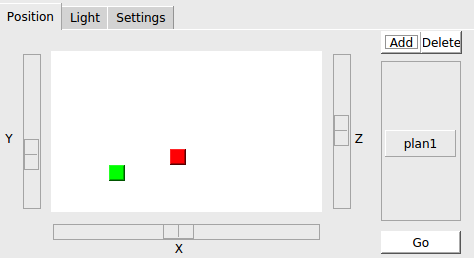
\includegraphics[width=0.9\linewidth]{0_Filer/Figuer/Position.png}
\caption{Position-tab}
\label{fig:GUI Position}
\end{figure}

\subsubsection{Light}
Light er den anden tab fra venstre mod højre, som kan ses i tab-widget menuen. Det er i denne tab, hvor interaktionen med lysstyring foretages. Selve vinduet er bygget op som en del af tab-widgetten i Displays's UI, men det er light.cpp, der står for behandlingen af interaktionerne, der sker i dette tab. 
Nedenfor ses et klassediagram for GUI'en, hvor klasserelationerne kan ses. Det fremgår af klasserelationerne, at Position som primære fil står for at hente data fra GUI'en og brugerens interaktionen med den, hvilket hovedsagligt foregår med signals \& slots. Signals \& slots er GUI'ens interne eventhandler. Når dette event sker, sendes dette signal til dette slot (funktion) som udfører det og det. QT er et eventbaseret system, så opbygningen af den er primært bestående af forståelsen for hvordan delelementer snakker sammen, eller snarer hvordan man får dem til at snakke sammen. Arv og pointerlogik spiller her en stor rolle.

\begin{figure}[H]
\centering
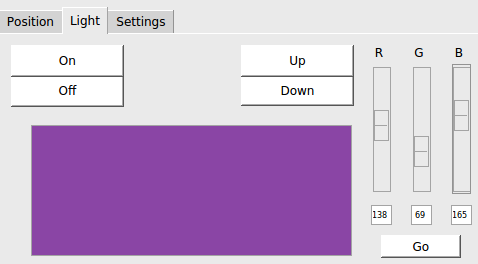
\includegraphics[width=0.9\linewidth]{0_Filer/Figuer/Light.png}
\caption{Light-tab}
\label{fig:GUI Light}
\end{figure}

\subsubsection{Settings}
Settings er den tredje tab fra venstre mod højre. Denne tab har til ansvar at sætte sensorindstillingerne. Disse sensorer indbefatter afstandssensor, bevælgelsessensor og lumensensor. Bevægelsessensoren og lumensensoren er helt simplistisk bestående af sliders som kan sættes til minumum, der beskriver tilstanden Off eller maksimum, der beskriver tilstande On. Når disse er On betyder det at sensorne er aktive og deres respons på virker udfaldsforløbet. Afstandssensoren er opbygget med af en spinbox, hvori man kan indstille hvilken afstand den skal registrere at et objekt er for tæt på. Dette er en heltalsværdi med minimum på 3 og maximum på 255 med enheden centimeter. Det er også i denne tab at kalibreringsknappen ”Calibrate” kan findes. Calibrate er noget brugeren kan benytte til at rette op på uoverensstemmelser i positionering hvis denne er skredet fra det forventet. Dette påbegynder en bevægelsesrutine og lagrer ved afslutning nogle calibreringsdata på de respektive slave PSoC'er, PSoC-XY og PSoC-Z.

\begin{figure}[H]
\centering
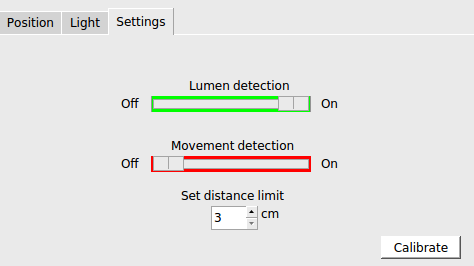
\includegraphics[width=0.9\linewidth]{0_Filer/Figuer/Settings.png}
\caption{Settings-tab}
\label{fig:GUI Position}
\end{figure}

\subsubsection{PlannerDialog og planner}
Plannerdialogboksen er den dialogboks der bringes frem, når man trykker på Add-knappen, hvis brugeren vælger at oprette en plan der skal gemmes. Dialogboksen indeholder et tekstfelt hvori navnet på planen indtastes. Der kan heri indtastes alle tegntyper begrænset til maksimalt 8-tegn. Dette antal er valgt for at de oprettede knapper har et navn det fylder maksimalt en linje med en skriftstørrelse, der vil være læsbar på et display af den størrelse der benyttes til dette produkt (480*272). Alt over 8-tegn ville kræve at skriftstørrelsen skulle være mindre eller der skulle laves linjeskift, hvilket ikke ville være hensigtsmæssigt. Indtastningen i indtastningsfeltet gøres vha. af det virtuelle keyboard, der befinder sig i den nederste halvdel af skærmen i dialogboksen. 

Keyboardet er ikke lavet af denne gruppe, men er blevet downloadet og implementeret fra "the Free Software Foundation". Keyboardet er dog blevet modificeret i størrelse og indtastningsvenlighed, og "Hide"-knappen der oprindeligt skulle benyttes til at skjule keyboardet er blevet gjort funktionsløst, da denne funktionalitet var unødvendig for dette produkt. For mere information om dette keyboard samt et downloadlink til det kan ses fra følgende reference\#. Under indtastningsfeltet kan findes en Ok- og Cancel-knap. Tryk på Ok-knappen opretter planen med det indtastede navn, hvorimod Cancel-knappen annulerer oprettelse af plan og returnere brugeren til den forhenværende brugerflade. For at undgå at navneløse planer bliver oprettet er Ok-knappen disablet indtil mindst et eller flere tegn indtastes i indtastningsfeltet. Der er en begrænsning på mængden af planer på 4, da dette var den maksimale mængde, der var plads til foruden knapstørrelsen skulle formindskes. Hvis en plan ønskes fjernet skal brugeren trykke på givne plan og trykke på Delete-knappen placeret ved siden af Add-knappen.

\begin{figure}[H]
\centering
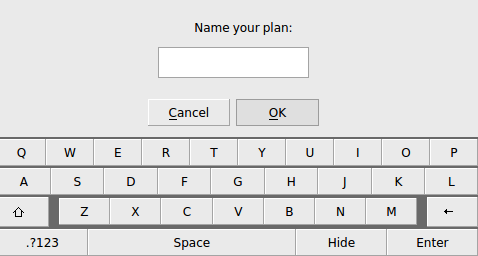
\includegraphics[width=0.9\linewidth]{0_Filer/Figuer/plannerDialog.png}
\caption{Settings-tab}
\label{fig:GUI Dialog}
\end{figure}

% 6.1.2.4 Klassebeskrivelser Devkit8000
\subsection{Klassebeskrivelse Devkit8000}

MainDisplay er den første UI, som åbnes, når applikationen startes og det eneste, som forbliver åbent. Det er applikationens primære UI-fil, hvor den hovedsaglige interaktion foretages og fungerer som bindeled for GUI'ens klasser. Denne QWidget indeholder en stor række af GUI'ens funktionaliteter da GUI'en blev opbygget i tabs i stedet for i seperate QWidgets. MainDisplay's UI-fil indeholder den grundlæggende funktionalitet, som er nødvendig for at oprette vinduet.
\newline

Nedenfor ses et klassediagram for GUI’en, hvor det fremgår, at MainDisplay er den ledende klasse med det UI, som de andre klasser bruges i. Det fremgår af klasserelationen, at MainDisplay som Main Window anvender GUI’ens resterende klasser, hvilket hovedsagligt foregår med signals \& slots. Position, Planner og Light har ikke deres egne QWidget klasser da de alle er bygget på MainDisplay QWidgeten, hvilket har resulteret i en stor samling af klasse i en fil.

\begin{figure}[H] \centering
    \fbox{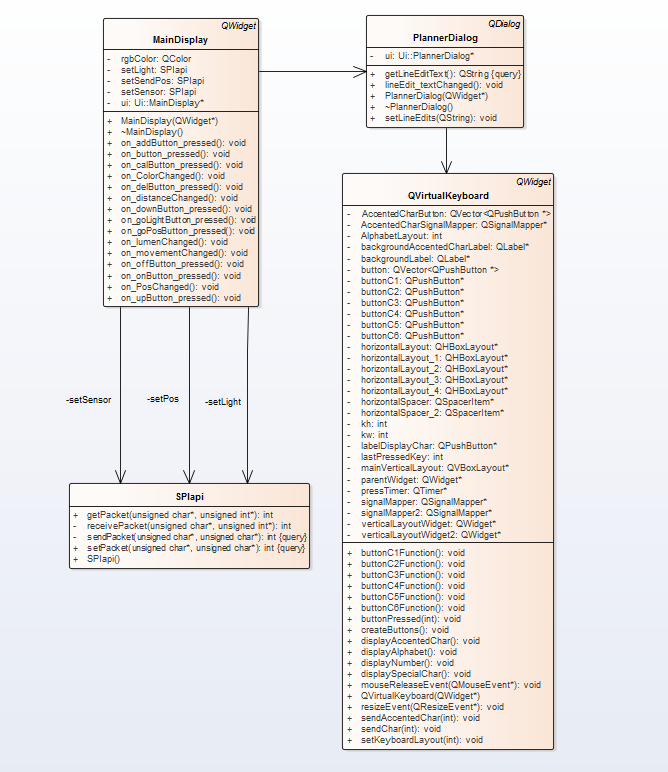
\includegraphics[width=0.95\textwidth]{0_Filer/Figuer/guiClassDia.png}}
    \caption{GUI klassediagram}
    \label{fig:GUI klassediagram}
\end{figure}

% 6.1.2.5 GUI repræsentationsbeskrivelse
\subsection{GUI repræsentationsbeskrivelse}

Klassen Position består af følgende filer:
\begin{itemize}
\item display.ui
\item position.cpp
\item maindisplay.h
\end{itemize}

display.ui er den UI-fil der indeholder de grafiske elementer der kodes for og denne UI-fil kræver sin tilhørende headerfil maindisplay.h. Source-filen position.cpp er der hvor al funktionalitet kodes.
\newline

GUI-filen repræsenterer et vindue bestående af følgende elementer:
\begin{itemize}

\item Tab Widget - Indeholder tre separate tabs: Position, Light og Settings.

\item Sliders (Position-tab) – Til indstilling af lampens position i X-, Y- og Z-aksen i trin mellem 0 og 255.

\item Go-knap (Position-tab) – Til at udsende sliderværdierne for X, Y og Z til bevægelse af lampe.

\item Add-knap (Position-tab) - Til åbne dialogboksen til oprettelse af en plan.

\item Sliders (Light-tab) - Til indstilling af farven der udsendes til lampen i trin mellem 0 og 255.

\item Trinbokse (Light-tab og Position-tab) - Til visning af sliders trinværdi.

\item Farvepalette (Light-tab) - Hvor indstillede farve vises, der forventes at blive vist på lysenhed.

\item On/Off-knapper (Light-tab) – On-knap til at sætte RGB-LED’erne på sidste lysindstilling forinden den blev slukket og Off-knap for at slukke lyset.

\item Up/Down-knapper (Light-tab) - Bruges til at flytte farvesliders enten op eller ned med 5 steps.

\item Labels – Position: X, Y og Z til identifikation af hvilken slider der kontrollerer hvilken akse. Light: R, G og B til identifikation af sliders for farverne rød, grøn og blå.

\item Plot – Et X-, Y-koordinatsystem til visualisering af lampens nuværende position (med grønt ikon) og dens kommende position (rødt ikon), hvis sliders er blevet flyttet.

\item Lumen slider (Settings-tab) - En slider til at sende en tænd- eller slukbesked til lyssensoren.

\item Movement slider (Setttings-tab) - En slider til at sende en tænd- eller slukbesked til bevægelsessensoren.

\item Distance spinbox (Settings-tab) - En spinbox der sætter den værdi hvorindenfor afstandssensoren sender en advarsel.

\end{itemize}

I constructoren til klassen MainDisplay sker opsætningen af GUI'en, når den startes. Her får vi komponenter fra UI'et til at kommunikere sammen med signals \& slots. Dette gøres vha. connect() metoder, så der kan emittes signaler, hvorefter de tilhørende slots kaldes. I dette specifikke kodeudsnit ses hvordan slidernes signaler er blevet sat op. Alle sliderne fra de tre tabs connectes samtidig. Position, Light og Settings er dermed klar til intern kommunikation forinden metoderne kaldes.

\begin{figure}[H]
\centering
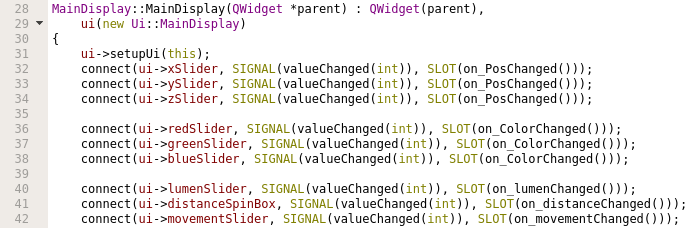
\includegraphics[width=0.9\linewidth]{0_Filer/Figuer/signalSlot.png}
\caption{Kodeudsnit af Signals \& Slots i MainDisplay's constructor}
\label{fig:signalSlot}
\end{figure}

{\centering \textbf{spi-api} \par}

\begin{table}[H]
    \centering
    \begin{tabular}{|l|}
    \hline
    \multicolumn{1}{|c|}{<<boundary>>} \\
    \multicolumn{1}{|c|}{\textbf{spi-api}} \\
    \hline
    \\
    \hline
    + txPacket(unsigned char* const, unsigned char* const) : int \\
    + rxPacket(unsigned char* const, unsigned int*) : int \\
    \hline
    \end{tabular}
    \caption{Klasse spi-api}
    \label{tab:classSpiApi}
\end{table}

\begin{labeling}{Attributter:}
\item[Ansvar:] At være et lag imellem \textit{applications}-laget og \textit{device driver}-laget ifa. et \textit{kernemodul} på DevKit8000 som står for SPI kommunikationen.
\item[Attributter:] Ingen.
\end{labeling}

\begin{labeling}{Beskrivelse:}
\item[int txPacket(unsigned char* const, unsigned char* const)]
\item[Parametre:] Modtager to unsigned char pointere som peger på hhv. kommandoen og dataen der skal sendes via SPI-netværket til PSoC master fra DevKit8000.
\item [Returværdi:] Retunere en int med værdien 0 ved succes ellers en negativ værdi i overenstemmelse med fejl-listen.
\item [Beskrivelse:] Metoden skal sende en kommando og dertilhørende data væredi som en pakke via SPI-netværket fra DevKit8000 til PSoC Master med en kommando og data.
\end{labeling}

\begin{labeling}{Beskrivelse:}
\item[int rxPacket(unsigned char* const, unsigned int*)]
\item[Parametre:] Modtager en unsigned char pointer og en unsigned int pointer som peger på hhv. kommandoen der skal sendes til, og dataen hvor retur værdien skal lageres, som sendes via SPI-netværket til PSoC master fra DevKit8000.
\item [Returværdi:] Retunere en int med værdien 0 ved succes ellers en negativ værdi i overenstemmelse med fejl-listen.
\item [Beskrivelse:] Metoden skal sende en data pakke med kommandoen og derefter aflæse retur data fra PSoC Master som lagers på den dertil angivet unsigned int pointer, via SPI-netværket fra DevKit8000 til PSoC Master og retur.
\end{labeling}

{\centering \textbf{Position} \par}

\begin{labeling}{Attributter:}
\item[Ansvar:] Tage imod brugerens valg af lampeposition ud fra sliderenes position i taben ved navn Position.
\item[Attributter:] qunt8 x\_: En unsigned 8-bit integer som bestemmer lampens x-værdi (til koordinatstyring). \\
quint8 y\_: En unsigned 8-bit integer som bestemmer lampens y-værdi (til koordinatstyring). \\
quint8 z\_: En unsigned 8-bit integer som bestemmer lampens z-værdi (til koordinatstyring).
\end{labeling}

\begin{labeling}{Beskrivelse:}
\item[struct setXYZ(quint8, quint8, quint8)]
\item [Parametre:] Unsigned int med x-værdi. \\
Unsigned int med y-værdi. \\
Unsigned int med z-værdi.
\item [Returværdi:] x, y og z’s sliderværdier til positionering.
\item [Beskrivelse:] En struct med ansvar for at sætte x-, y- og z-værdierne som skal sendes videre så motorerne kan styres i tre dimensioner.
\end{labeling}

\begin{labeling}{Beskrivelse:}
\item[void on\_PosChanged()]
\item[Parametre:] Ingen.
\item [Returværdi:] Ingen.
\item [Beskrivelse:] Metoden er et slot til sliderReleased() signaler og kaldes ved sliderReleaseEvent
(når en slider slippes efter brug). Den sætter koordinatværdier ud fra sliderpositioner i trin mellem 0 og 255. Disse sendes videre til lampepositionering.
\end{labeling}

\begin{labeling}{Beskrivelse:}
\item[void on\_calButton\_clicked()]
\item[Parametre:] Ingen.
\item [Returværdi:] Ingen.
\item [Beskrivelse:] Kalibrerer system ved først at set X, Y og Z til den maksimale værdi muligt og returnerer til positionen før kalibrering når opgaven er tilendebragt.
\end{labeling}

\begin{labeling}{Beskrivelse:}
\item[Display::\char`\~Display()]
\item[Parametre:] Ingen
\item [Returværdi:] Ingen
\item [Beskrivelse:] Destructor til nedlæggelse af det grafiske interface, når den kaldes
\end{labeling}

\begin{labeling}{Beskrivelse:}
\item[bool getCalStatus()]
\item[Parametre:] Ingen
\item [Returværdi:] En true eller false der beskriver om kalibrering forløber korrekt.
\item [Beskrivelse:] Hvis kalibrering forløber fejlfrit vil true blive returneret og ellers returneres false. En information, der kan bruges til fejlhåndtering.
\end{labeling}

\begin{labeling}{Beskrivelse:}
\item[void setStatusLine(const QString)]
\item[Parametre:] Et tekststykke der beskriver sidste handling udført.
\item [Returværdi:] Ingen.
\item [Beskrivelse:] En statuslinje der udskriver hvad status for systemet er lige nu.
\end{labeling}

{\centering \textbf{Light} \par}

\begin{labeling}{Attributter:}
\item[Ansvar:] Indstille lysets farve og intensitet for lampen.
\item[Attributter:] quint8 red\_: En unsigned 8-bit integer som bestemmer lampens røde farveintensitet.\\
quint8 green\_: En unsigned 8-bit integer som bestemmer lampens grønne farveintensitet. \\
quint8 blue\_: En unsigned 8-bit integer som bestemmer lampens blå farveintensitet.
\end{labeling}

\begin{labeling}{Beskrivelse:}
\item[struct setSliders(quint8, quint8, quint8)]
\item[Parametre:] Unsigned 8-bit integer med red\_. Unsigned 8-bit integer med green\_. Unsigned 8-bit integer med blue\_.
\item [Returværdi:] En struct med ansvar for at sætte R-, G- og B-værdierne, som skal sendes videre så RGB’ernes farveniveauer kan styres.
\item [Beskrivelse:] En struct med ansvar for at sætte red-, green- og blue-værdierne, som skal sendes videre til lampens RGB-LED’ers farve og lysintensitet. Alle farverne bestemmes med en trinværdi mellem 0 og 255.
\end{labeling}

\begin{labeling}{Beskrivelse:}
\item[void on\_upButton\_clicked()]
\item[Parametre:] Ingen.
\item [Returværdi:] Ingen.
\item [Beskrivelse:] Øger lampens lysintensitet ved at lægge en til alle farver (rød, grøn og blå), ved klik på Up-knappen i GUI’ens Light-tab.
\end{labeling}

\begin{labeling}{Beskrivelse:}
\item[void on\_downButton\_clicked()]
\item[Parametre:] Ingen.
\item [Returværdi:] Ingen.
\item [Beskrivelse:] Sænker lampens lysintensitet ved trække en fra alle farver (rød, grøn og blå), ved klik på Down-knappen i GUI’ens Light-tab.
\end{labeling}

\begin{labeling}{Beskrivelse:}
\item[void on\_onButton\_clicked()]
\item[Parametre:] Ingen.
\item [Returværdi:] Ingen.
\item [Beskrivelse:] Tænder lampens lys med sidst benyttede intensitet, ved klik på On-knappen i GUI’ens Light-tab.
\end{labeling}

\begin{labeling}{Beskrivelse:}
\item[void on\_offButton\_clicked()]
\item[Parametre:] Ingen.
\item [Returværdi:] Ingen.
\item [Beskrivelse:] Slukker lampens lys ved klik på Off-knappen i GUI’ens Light-tab.
\end{labeling}

\begin{labeling}{Beskrivelse:}
\item[void updatePalette(QColor\&)]
\item[Parametre:] Reference til farve som Color Preview sættes med.
\item [Returværdi:] En struct med ansvar for at sætte R-, G- og B-værdierne som skal sendes videre så RGB’ernes farveniveauer kan styres.
\item [Beskrivelse:] En struct med ansvar for at sætte red-, green- og blue-værdierne, som skal sendes videre til lampens RGB-LED’ers farve og lysintensitet. Alle farverne bestemmes med en trinværdi mellem 0 og 255.
\end{labeling}

\begin{labeling}{Beskrivelse:}
\item[bool lightSens()]
\item[Parametre:] Ingen.
\item [Returværdi:] True hvis lyssensorens input skal behandles eller false hvis kommunikation med lyssensor er deaktiveret.
\item [Beskrivelse:] Der vil her blive angivet og hvor vidt kommunikation med lyssensoren vil blive behandlet.
\end{labeling}

\subsection{GUI modultest}
Der er blevet lavet en række forskellige test på GUI'en for at sikre at alle funktionerne har de korrekte funktionaliteter. Koden indeholder mange metoder og interne signaler der skal sendes rigtigt hele vejen igennem systemet for at sikre at resten af systemet vil kunne bruge de udsendte data. GUI test er primært blevet fortaget med QDebugger som bliver brugt til at udskrive data og tekststrenge for at de kunne følge kodens forløb. \newline

\begin{table}[H]
\begin{tabular}{|l|l|}\hline
\textbf{Test} & Positionsindstilling ved sliderændringer \\\hline

\textbf{Testbeskrivelse} & \multicolumn{1}{|m{11.5cm}|}{Det testes, om ændring af X-, Y- og Z-sliders positioner sætter nogle værdier og om de bliver sendt korrekt ved tryk på Go-knap.  QDebug() bruges til at udskrive positionsværdierne i metoden on\_PosChanged(), der kaldes ved valueChanged(int).} \\\hline


\textbf{Input} & \multicolumn{1}{|m{11.5cm}|}{Sliders positioner ændres til hhv. 255, 255, 255. Derefter trykkes Go-knappen ned og slippes igen.} \\\hline

\textbf{Output} & \multicolumn{1}{|m{11.5cm}|}{ Sliderpositionen og nuværende position vil ændre sig til "255, 255, 255", blive udskrevet og de negative kommandokoder vil blive returneret som fejlkoder (X=16, Y=17, Z=32).} \\\hline

\textbf{Resultat} & \multicolumn{1}{|m{11.5cm}|}{ OK} \\\hline

\end{tabular}
\end{table}

\begin{figure}[H]
\centering
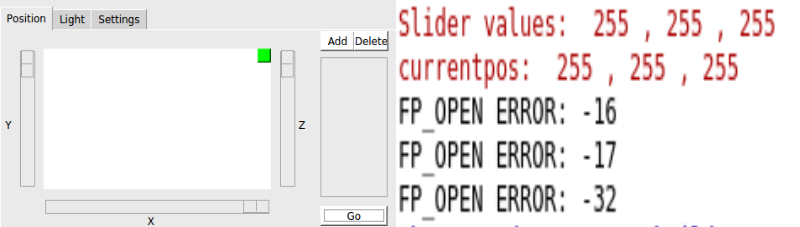
\includegraphics[width=0.9\linewidth]{0_Filer/Figuer/testPosition.png}
\caption{Debug output ved sliderværdierne (X, Y, Z): 255, 255, 255, den sendte værdi currentpos: 255, 255, 255 og negative sendte kommandoer.}
\label{fig:testPosition}
\end{figure}


\begin{table}[H]
\begin{tabular}{|l|l|}\hline
\textbf{Test} & Lysindstilling ved sliderændringer \\\hline

\textbf{Testbeskrivelse} & \multicolumn{1}{|m{11.5cm}|}{Det testes, om ændring af R-, G- og B-sliders positioner sætter nogle værdier og om de bliver sendt korrekt ved tryk på Go-knap.  QDebug() bruges til at udskrive positionsværdierne i metoden on\_ColorChanged(), der kaldes ved valueChanged(int).} \\\hline

\textbf{Input} & \multicolumn{1}{|m{11.5cm}|}{Sliders positioner ændres til hhv. 255, 255, 255. Derefter trykkes Go-knappen ned og slippes igen.} \\\hline

\textbf{Output} & \multicolumn{1}{|m{11.5cm}|}{ Sliderpositionen og sendte lysværdi vil ændre sig til "255, 255, 255", blive udskrevet og de negative kommandokoder vil blive returneret som fejlkoder (R=48, G=49, B=50).} \\\hline

\textbf{Resultat} & \multicolumn{1}{|m{11.5cm}|}{ OK} \\\hline

\end{tabular}
\end{table}

\begin{figure}[H]
\centering
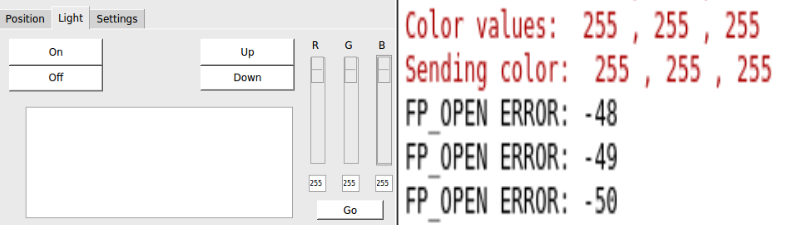
\includegraphics[width=0.9\linewidth]{0_Filer/Figuer/testLight.png}
\caption{Debug output ved sliderværdierne Color values (R, G, B): 255, 255, 255, den sendte værdi Sending color: 255, 255, 255 og negative sendte kommandoer.}
\label{fig:testLight}
\end{figure}



\begin{table}[H]
\begin{tabular}{|l|l|}\hline
\textbf{Test} & Sensorindstilling ved slider og spinboxændringer \\\hline

\textbf{Testbeskrivelse} & \multicolumn{1}{|m{11.5cm}|}{Det testes, om ændring af Movementslider og Lumensensor samt Distancespinbox bliver sendt videre med spi kommandoer.} \\\hline

\textbf{Input} & \multicolumn{1}{|m{11.5cm}|}{Sliders position for Movement og Lumen ændres fra Off til On. Derefter ændres Distancespinboxværdien til 4.} \\\hline

\textbf{Output} & \multicolumn{1}{|m{11.5cm}|}{ Sliderpositioner for Lumen og Movement ændres til On, status bliver udskrevet og de negative kommandokoder vil blive returneret som fejlkoder (R=48, G=49, B=50).} \\\hline

\textbf{Resultat} & \multicolumn{1}{|m{11.5cm}|}{ OK} \\\hline

\end{tabular}
\end{table}

\begin{figure}[H]
\centering
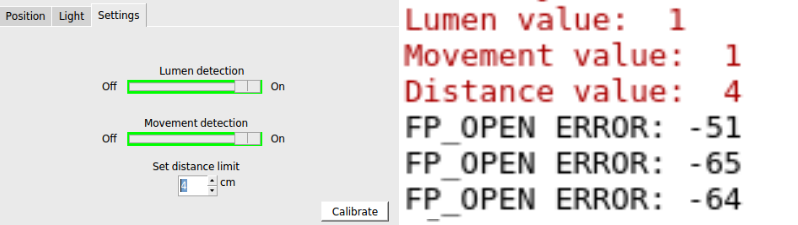
\includegraphics[width=0.9\linewidth]{0_Filer/Figuer/testSettings.png}
\caption{Debug output ved sliderværdierne Lumen value: 1, Movement value: 1, spinboxværdien Distance value: 4 og negative sendte kommandoer.}
\label{fig:testSettings}
\end{figure}



\begin{table}[H]
\begin{tabular}{|l|l|}\hline
\textbf{Test} & Oprettelse af plan \\\hline

\textbf{Testbeskrivelse} & \multicolumn{1}{|m{11.5cm}|}{Det testes, om der kan oprettes en plan og de korrekte værdier gemmes.} \\\hline

\textbf{Input} & \multicolumn{1}{|m{11.5cm}|}{Sliderposition for X, Y og Z ændres til "255, 255, 255" og R, G, og B ændres til "255, 0, 0". Der trykkes dernæst op Add-knappen, et navn indtastes i dialogboksen der fremvises på skærmen og Ok-knappen trykkes.} \\\hline

\textbf{Output} & \multicolumn{1}{|m{11.5cm}|}{Plannens positionsvædier sættes til "255, 255, 255" og lysværdierne sættes til "255, 0, 0". Disse værdier udskrives i debuggeren.} \\\hline

\textbf{Resultat} & \multicolumn{1}{|m{11.5cm}|}{ OK} \\\hline

\end{tabular}
\end{table}

\begin{figure}[H]
\centering
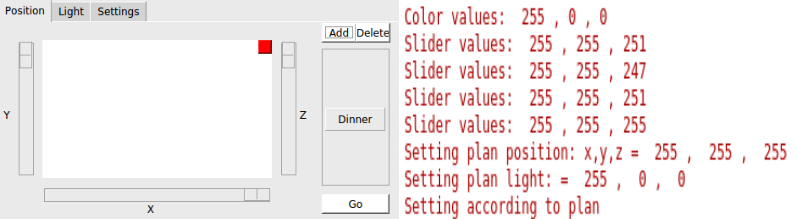
\includegraphics[width=0.9\linewidth]{0_Filer/Figuer/testMakePlan.png}
\caption{Debug output ved satte plan X, Y og Z Setting plan position: (255, 255, 255), lyset R, G, B Setting plan Light (255, 0, 0) og Setting according to plan}
\label{fig:testmakePlan}
\end{figure}
